\subsection{Les newsgroups}
\label{newsgroups}
\subsubsection{Présentation}
Le BR fournit aux élèves un service de \emph{newsgroups}, souvent surnommé \guillemotleft~les br~\guillemotright . Ils fonctionnent un peu comme un
forum : chacun peut poster une annonce, poser une question,
 répondre à un sujet posté par un autre élève\ldots\
Ils sont très utiles pour faire de la pub pour une activité
organisée par un binet, poser une question en cas de problème, ou
tout simplement savoir ce qu'il se passe sur le platâl. Pour qu'ils
puissent remplir pleinement ce rôle, le BR a édicté un certain
nombre de règles que les newsmestres sont chargés de faire
respecter.

\subsubsection{Les règles}
\begin{itemize}
 \item Pas d'insultes, attaques personnelles, calomnies et autres.
 \item Ne pas dissimuler son identité, et donc utiliser une adresse mail valide
       et un pseudo qui permet de t'identifier par l'intermédiaire du TOL. Poster depuis un ordinateur de binet ou de bar section est ainsi fortement déconseillé (sauf sur les br.binet.* ou br.section.* correspondants, mais mettre son nom en fin de message reste conseillé et poli).
 \item Pour que les {\it br} restent lisibles, faire des crossposts propres (\emph{cf.} infoBR p11).
 \item Dans le même ordre d'idée, poster sur le forum adapté:
       les petites annonces vont sur le \ngname{br.pa} et nulle part ailleurs,
       seules les questions concernant directement le BR ont leur place sur le \ngname{br.binet.br}
       (pour les questions d'informatique il y a les \ngname{br.informatique.*}).
 \item Eviter de troller\footnote{poster des messages provocateurs et non constructifs dans le seul but
       d'engendrer des polémiques\ldots ou tout simplement entrer dans le jeu de celui qui te provoque
       et poster une centaine de messages inutiles en quelques dizaines de minutes ;)} abusivement
       (sauf sur \ngname{br.binet.polemix} qui sert à ça ;-))
 \item Garder son calme (ou éviter de poster), mieux vaut une explication dans la vraie vie
       que par {\it br} interposé.
\end{itemize}

\subsubsection{Les différents newsgroups de frankiz}
Frankiz héberge un grand nombre de newsgroups (plus de 200\dots ), mais il est probable qu'ils ne t'intéressent pas tous.

Il est trés important  que tu sois abonné au br suivants :
\begin{itemize}
\item[\ngname{br.eleves} :] posts généraux (pas de petites annonces, br.pa est là pour ça ! ), intéressant potentiellement un grand nombre d'élèves. C'est "LE" br que tu dois lire.
	 
\item[\ngname{br.pa} :] pour les petites annonces. Tu cherches un bidulle tu écris "Ping Bidule". Tu as en a ta possession un machin que tu veux rendre à son proprétaire, vendre, partager, etc... tu écris "Pong Machin". C'est "LE" lieu, et le seul, pour les annonces.

\item[\ngname{br.promo.*} :] pour les posts ne concernant à priori qu'une seule promo (Rouje, Jone ou Oranje).
	 
 \item[\ngname{br.enseignement.*} :] pour tout ce qui a trait à l'enseignement (un DM, un message aux délégués d'enseignement...) concernant ta promo (rouje ou jone).	 
 
 \item[\ngname{br.section.ta\_section\_sportive} :] le \emph{newsgroup} de ta section.                                        Utile pour savoir ce qu'il s'y passe et planifier les activités.

\item[\ngname{br.informatique.media.request} :] pour les films, les musiques. (ex : Ping Star Wars)

\item[\ngname{br.informatique.nouveautés} :] pour les dernièrs films, séries, albums. (un de br les plus lus)

\item[\ngname{br.binet.br} :] comme son nom l'indique, il s'agit du newsgroup du binet réseau. À utiliser pour les questions ayant un lien \emph{direct} avec le BR.

 \item[\ngname{br.informatique.windows/linux/mac} :] selon ton OS, quand tu as un problème, ou besoin d'une astuce, ou d'un logiciel.

 \item[\ngname{br.kes} :] le newsgroup de la Kès. Il sert essentiellement à la Kès pour faire une annonce, ou aux élèves pour poser une question aux fruits de kessiers (note: il n'est pas non plus interdit de se déplacer à la Kès pour poser ta question directement)

\end{itemize}

Pour le reste, voila une liste de quelques \emph{newsgroups} utiles :
\begin{itemize}
\item[\ngname{br.binet.ton\_binet} :] chaque binet a son \emph{newsgroup} (s'il en a demandé un). Il sert le plus souvent pour la communication interne du binet, ses annonces ou à poser une question au dit binet. Dans le cas d'un nouveau binet, le BR peut lui créer un \emph{newsgroup}, mais uniquement après que le binet a été créé dans les règles à la Kès.

\item[\ngname{br.binet.polemix} :] le forum pour troller (un troll est une trés longue discussion qui dégénère) par excellence.
                          
\item[\ngname{br.communauté.*} :] les newsgroups de différentes communautés (religieuses, musicales, géographiques ou autres)

\item[\ngname{br.test} :] quand tu veux tester un truc sur les newsgroups, viens le faire ici plutôt que de pourrir un br utile. La tradition est  d'y laisser une blague après y avoir posté.

 \item[\ngname{br.trash} :] pour les craquages.
 
 \item[\ngname{public.*} :] les \emph{newsgroups accessibles à l'ensemble du personnel de l'école}.
                   Il y a peu de messages postés, mais ils peuvent parfois se réveler utiles.
\end{itemize}

Il arrive parfois que certains \emph{newsgroups} temporaires soient créés pour des évènements particuliers (campagne Kès). Leur création sera annoncée
le plus souvent sur \fkz ou sur le \ngname{br.eleves}.

\subsubsection{Autres newsgroups}
Le site \urllink{polytechnique.org} dispose de son propre service de \emph{newsgroups}. Il sont
accessibles à tous les polytechniciens, qu'ils soient actuellement sur le campus ou membres de
promos précédentes. Pour plus d'informations, consulte \server{www.polytechnique.org}.

Il est aussi possible d'accéder à certains \emph{newsgroups} extérieurs à l'école via \server{polynews}. Ce serveur de la DSI est synchronisé avec
l'extérieur. Si tu cherches un \emph{newsgroup} qui ne s'y trouve pas, n'hésite pas à demander aux newsmestres (cf section suivante).

\subsubsection{Les newsmestres}
Les newsmestres sont les membres du BR chargés de l'administration et de la modération des \emph{newsgroups}. Leur but est de maintenir les
\emph{newsgroups} dans un état correct, pour que tout le monde puisse en profiter et trouver ce qu'il y cherche. Ne prends donc pas une remarque de
leur part comme une attaque personnelle\dots

Pour les contacter: \mail{news@frankiz.polytechnique.fr}.



%\setcounter{page}{11}

\subsubsection{Poster sur plusieurs newsgroups\dots }



Il se peut qu'un jour tu veuilles annoncer un grand événement sur les \emph{newsgroups}, et que pour ceci tu aies envie de poster ton message sur
plusieurs \emph{newsgroups}. Alors avant de commencer à poster sur un \emph{newsgroup}, faire copier-coller, poster sur le \emph{newsgroup} suivant,
etc., lis ce qui suit et apprend à gagner du temps, et simplifier ta vie et celle de tes camarades.

\paragraph{Qu'est-ce qu'un crosspost ?}
Un crosspost permet de poster le même message sur différents \emph{newsgroups}, et de renvoyer toutes les réponses sur le même \emph{newsgroup}, quel
que soit le \emph{newsgroup} sur lequel elles ont été postées.

\paragraph{Avantage d'un crosspost}
\begin{itemize}
 \item Toutes les réponses que les gens te font sont centralisées sur le même forum,
       ce qui t'évite de perdre du temps à lire des réponses disséminées
       sur les différents forums où tu as posté.
       De plus, ceux qui te répondent peuvent eux aussi lire facilement toutes les réponses
       que tu as déjà reçues.
 \item Sur certains clients news, il suffit de lire le message cross-posté sur un forum
       pour qu'il soit marqué comme lu sur tous les autres forums où il a été posté,
       ce qui évite ainsi aux gens de devoir lire plusieurs fois le même message.
 \item Cela t'évite de recevoir comme réponse un \guillemotleft~RTFIBRp11\footnote{Read The Fucking InfoBR page 11 :
       Lis Le Putain d'InfoBR page 11. Pour des raisons historiques, le cross-post est décrit à la page 11
       de l'InfoBR, c'est à dire cette page.}~\guillemotright  hargneux de la part d'un(e) newsmestre.
\end{itemize}

\paragraph{Comment faire un crosspost ?}
Il suffit de mettre dans le premier en-tête (\lien{Groupe de discussion} ou \lien{Newsgroup}) la liste de tous les \emph{newsgroups} où tu veux
poster, séparés par des virgules. \emph{Exemple :} \ngname{br.eleves, br.lose, br.binet.bob, br.promo.rouje}

Il faut ensuite mettre dans l'en-tête \lien{Transférer à} (ou \lien{Follow-up to}) le \emph{newsgroup} où tu veux que les réponses apparaissent. Si
tu n'a pas ces en-tête, sous Outlook Express va dans \lien{Affichage} et clique sur \lien{Tous les en-têtes} quand tu écris ton message, sous
Thunderbird, cliques sur la gauche de la deuxième ligne et sélectionne \lien{Faire suivre à :} dans le petit menu déroulant. Attention, ce doit être
l'un des \emph{newsgroups} où tu postes le message.
Voir par exemple les captures d'écran pour \app{Thunderbird} et \app{Outlook Express}.\\

\noindent\begin{tabular}{cc}
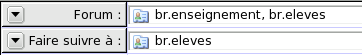
\includegraphics[width=0.45\textwidth]{images/cross_post_TB}
     & 
\includegraphics[width=0.45\textwidth]{images/cross_post_OE} \\
Thunderbird & Outlook Express
\end{tabular}
\vskip 12pt

C'est bien plus simple que d'envoyer successivement ton message sur tous les \emph{newsgroups}, et la centralisation des réponses permet de conserver
un peu de clarté sur les \emph{newsgroups}, tout en te facilitant la vie. Que des avantages donc!
